\documentclass[a4paper,11pt]{article}

%==============================================================================
% PACKAGES & CONFIGURATION
%==============================================================================

% Encoding & Language
\usepackage[utf8]{inputenc}
\usepackage[T1]{fontenc}
\usepackage[english]{babel}

% Page Layout & Typography
\usepackage[margin=2.5cm]{geometry}
\usepackage{helvet} % Modern Sans-Serif font
\renewcommand{\familydefault}{\sfdefault}
\usepackage{microtype} % Better character protrusion & kerning

% Paragraph spacing (optional but improves readability)
\setlength{\parskip}{0.5em}
\setlength{\parindent}{0pt}

% Colors (Unifonic Inspired)
\usepackage{xcolor}
\definecolor{UniGreen}{RGB}{0, 180, 120}     % Main Brand Color
\definecolor{UniDark}{RGB}{30, 35, 40}       % Dark Slate
\definecolor{UniLight}{RGB}{245, 247, 249}   % Light Background
\definecolor{AlertRed}{RGB}{220, 53, 69}     % Alert Color
\definecolor{CodeBg}{RGB}{250, 250, 250}

% Graphics & TikZ
\usepackage{graphicx}
\usepackage{tikz}
\usetikzlibrary{shapes, arrows.meta, positioning, shadows, calc, backgrounds, fit}

% Boxes and Code
\usepackage[most]{tcolorbox}
\usepackage{listings}
\usepackage{fontawesome5} % For icons

% Typography & Tables
\usepackage{titlesec}
\usepackage{booktabs}
\usepackage{array}
\usepackage{enumitem}

% Float control
\usepackage{float}

% Header/Footer
\usepackage{fancyhdr}
\pagestyle{fancy}
\fancyhf{}
\lhead{\textbf{\textcolor{UniGreen}{DataBug AI}}}
\rhead{\textcolor{UniDark}{Team CSIS}}
\cfoot{\thepage}
\renewcommand{\headrulewidth}{1pt}
\renewcommand{\headrule}{\hbox to\headwidth{\color{UniGreen}\leaders\hrule height \headrulewidth\hfill}}

% Section Styling
\titleformat{\section}
{\color{UniDark}\Large\bfseries}
{\color{UniGreen}\thesection\hspace{0.5em}}{0em}{}[\titlerule]

\titleformat{\subsection}
{\color{UniDark}\large\bfseries}
{\color{UniGreen}\thesubsection\hspace{0.5em}}{0em}{}

% Custom Code Style
\lstdefinelanguage{json}{
    basicstyle=\small\ttfamily,
    stringstyle=\color{UniGreen},
    keywordstyle=\color{blue!60!black},
    backgroundcolor=\color{CodeBg},
    frame=single,
    rulecolor=\color{black!10},
    breaklines=true,
    showstringspaces=false,
    commentstyle=\color{gray}
}

\lstset{
    language=json,
    basicstyle=\small\ttfamily,
    backgroundcolor=\color{CodeBg},
    frame=single,
    rulecolor=\color{black!10},
    breaklines=true,
    showstringspaces=false,
}

% Hyperlinks (loaded near the end of the preamble)
\usepackage{hyperref}
\hypersetup{
    colorlinks=true,
    linkcolor=UniGreen,
    urlcolor=UniDark,
    citecolor=UniGreen,
    pdfauthor={Team CSIS},
    pdftitle={DataBug AI - Data-Aware Intelligent Bug Triage}
}

% Table of contents depth (if you add a ToC)
\setcounter{tocdepth}{2}

%==============================================================================
% DOCUMENT CONTENT
%==============================================================================
\begin{document}

%--- TITLE PAGE ---
\begin{titlepage}
    \thispagestyle{empty}
    \begin{center}
        \vspace*{3cm}
        
        % Logo Construction
        
\begin{tikzpicture}
            \node[circle, fill=UniGreen, minimum size=2cm] (c) {};
            \node[text=white] at (c) {\Huge \faBug};
            \node[right=0.5cm of c, text=UniDark, font=\fontsize{40}{50}\bfseries] {DataBug AI};
        \end{tikzpicture}
        
        \vspace{1.5cm}
        {\Huge \textbf{Data-Aware Intelligent Bug Triage}}\\[0.5cm]
        {\Large The Immune System for CPaaS Support Infrastructure}
        
        \vspace{2cm}
        \begin{tcolorbox}[colback=UniLight, colframe=UniGreen, width=12cm, arc=5mm]
            \centering
            \textbf{\Large Team CSIS}\\
            \vspace{0.2cm}
            Unifonic AI Hackathon 2025
        \end{tcolorbox}
        
        \vspace{4cm}
        \textbf{Selected Tracks:}\\
        \vspace{0.3cm}
        Track 5: Automated Data Pipeline Validation\\
        Track 4: Bug Triage Automation
        
        \vfill
    \end{center}
\end{titlepage}

% Optional: Table of Contents
\tableofcontents
\newpage

%--- EXECUTIVE SUMMARY ---
\section*{Executive Summary}
\addcontentsline{toc}{section}{Executive Summary}

\begin{tcolorbox}[colback=UniLight, colframe=UniGreen, title=\textbf{The Core Insight}]
Research shows that \textbf{72\% of data quality issues} are discovered only after they have affected business decisions. For data-intensive organizations like Unifonic processing \textbf{10B+ transactions}, a single silent schema drift can cascade into hundreds of support tickets.
\end{tcolorbox}

\vspace{0.5cm}
\textbf{DataBug AI} is an open-source platform that revolutionizes bug triage by making it \textbf{data-pipeline-aware}. We bridge the gap between Data Engineering and Customer Support by automatically correlating incoming bug reports with upstream data quality incidents.

\vspace{0.5cm}
\begin{center}
    \begin{tabular}{p{0.45\textwidth} p{0.45\textwidth}}
        \toprule
        \textbf{Track Name} & \textbf{Weight in Solution} \\
        \midrule
        \textbf{Track 4:} Bug Triage Automation & 50\% (Symptom Management) \\
        \textbf{Track 5:} Data Pipeline Monitoring & 50\% (Root Cause Detection) \\
        \bottomrule
    \end{tabular}
\end{center}

%--- PROBLEM STATEMENT ---
\section{Problem Statement: The Hidden Connection}

\subsection{The Data Quality Crisis}
Data issues rarely stay contained. They propagate downstream, manifesting as "bugs" in dashboards, APIs, and mobile apps.

\vspace{0.5cm}
\begin{figure}[htbp]
    \centering
    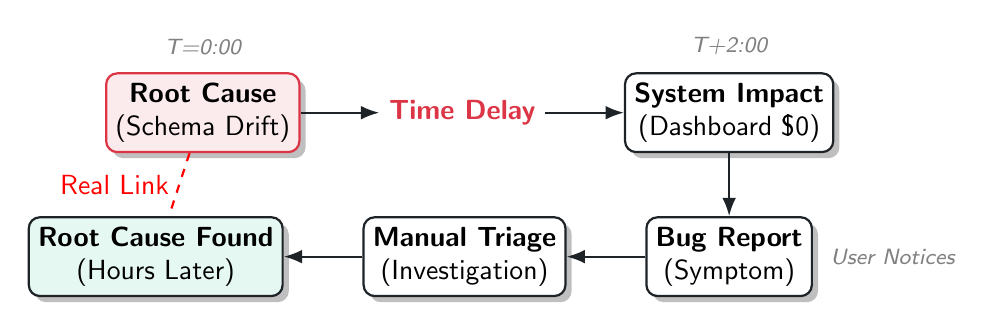
\begin{tikzpicture}[
        node distance=0.8cm and 1cm,
        box/.style={rectangle, draw=UniDark, thick, rounded corners, minimum height=1cm, align=center, fill=white, drop shadow},
        arrow/.style={-Latex, thick, UniDark},
        time/.style={font=\footnotesize\itshape, color=gray}
    ]
        % Nodes
        \node[box, fill=AlertRed!10, draw=AlertRed] (root) {\textbf{Root Cause}\\(Schema Drift)};
        \node[right=of root, font=\bfseries\color{AlertRed}] (delay) {Time Delay};
        \node[box, right=of delay] (impact) {\textbf{System Impact}\\(Dashboard \$0)};
        \node[box, below=of impact] (report) {\textbf{Bug Report}\\(Symptom)};
        \node[box, left=of report] (triage) {\textbf{Manual Triage}\\(Investigation)};
        \node[box, left=of triage, fill=UniGreen!10] (fix) {\textbf{Root Cause Found}\\(Hours Later)};

        % Arrows
        \draw[arrow] (root) -- (delay);
        \draw[arrow] (delay) -- (impact);
        \draw[arrow] (impact) -- (report);
        \draw[arrow] (report) -- (triage);
        \draw[arrow] (triage) -- (fix);
        
        % Annotations
        \node[time, above=0.1cm of root] {T=0:00};
        \node[time, above=0.1cm of impact] {T+2:00};
        \node[time, right=0.1cm of report] {User Notices};
        
        % Connect root to fix
        \draw[dashed, red, thick] (root) -- (fix) node[midway, left] {Real Link};
    \end{tikzpicture}
    \caption{The Disconnected Workflow: Why 50 tickets are filed for 1 data issue.}
\end{figure}

\subsection{Why Current Tools Fail}
\begin{itemize}[label=\textcolor{UniGreen}{\faTimesCircle}]
    \item \textbf{Data Tools (Great Expectations):} Alert on data, but don't see the support tickets.
    \item \textbf{Triage Tools (Jira):} See the tickets, but don't know the data pipeline is broken.
\end{itemize}

%--- SOLUTION ARCHITECTURE ---
\section{Solution Architecture}

DataBug AI sits as a middleware brain between the Data Layer and the Support Layer.

\vspace{0.5cm}
\begin{figure}[htbp]
    \centering
    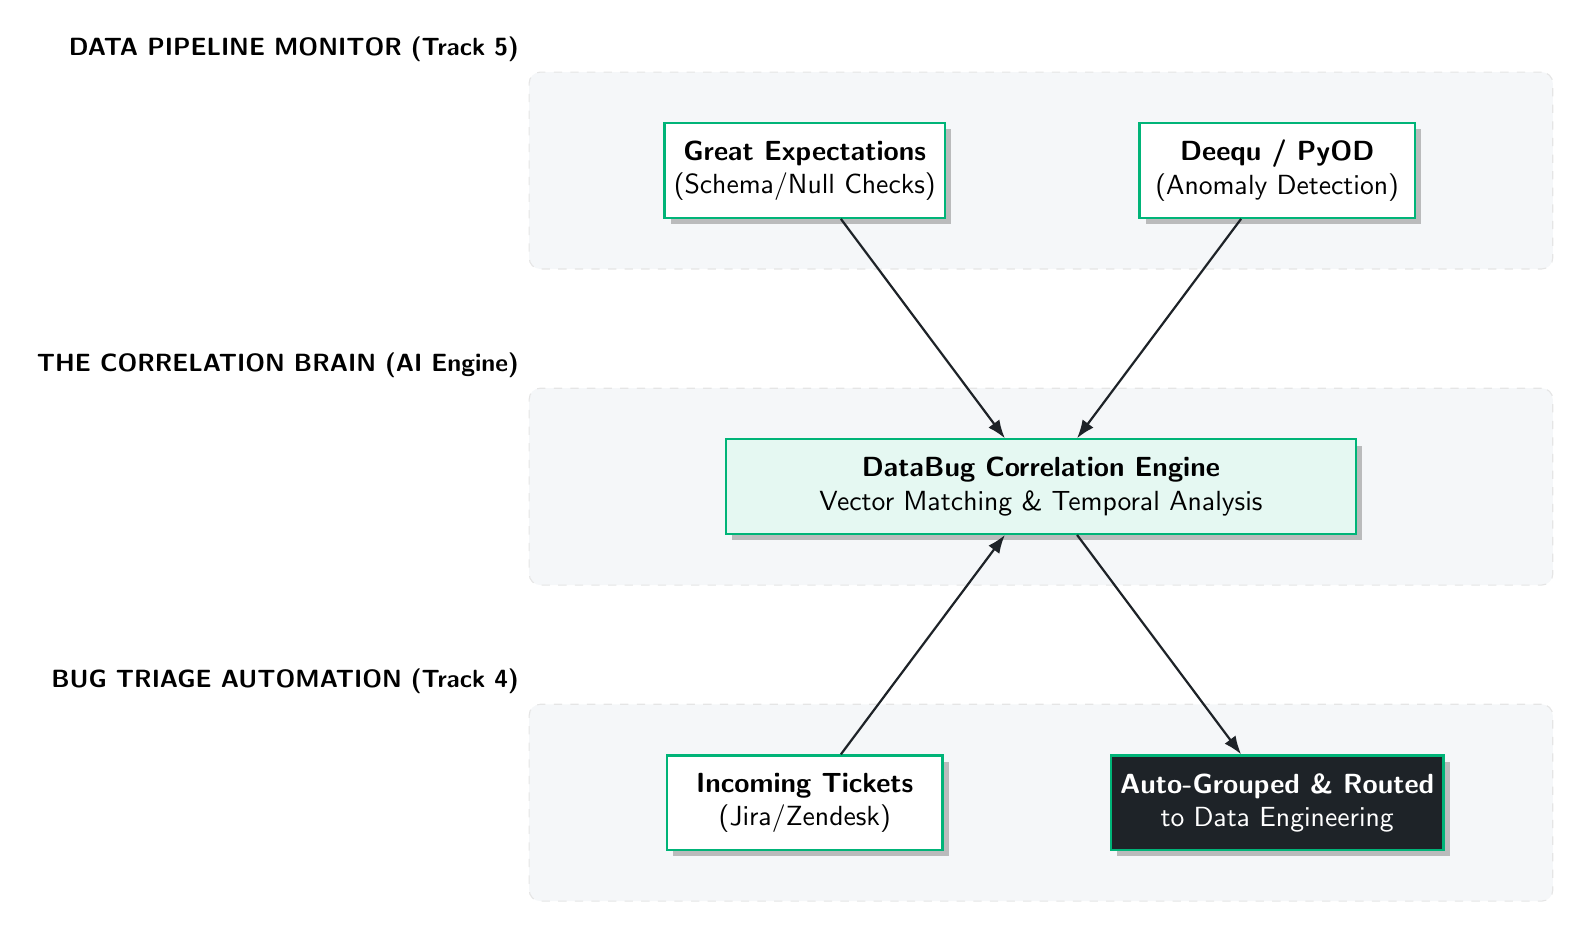
\begin{tikzpicture}[
        node distance=1.5cm,
        layer/.style={rectangle, draw=gray!20, fill=UniLight, dashed, minimum width=13cm, minimum height=2.5cm, rounded corners},
        comp/.style={rectangle, draw=UniGreen, thick, fill=white, minimum width=3.5cm, minimum height=1.2cm, align=center, drop shadow},
        link/.style={-Latex, thick, color=UniDark}
    ]
        % --- LAYERS ---
        \node[layer] (l1) {};
        \node[above left] at (l1.north west) {\small \textbf{DATA PIPELINE MONITOR (Track 5)}};
        
        \node[layer, below=1.5cm of l1] (l2) {};
        \node[above left] at (l2.north west) {\small \textbf{THE CORRELATION BRAIN (AI Engine)}};
        
        \node[layer, below=1.5cm of l2] (l3) {};
        \node[above left] at (l3.north west) {\small \textbf{BUG TRIAGE AUTOMATION (Track 4)}};

        % --- COMPONENTS ---
        % Layer 1
        \node[comp] (gx) at ([xshift=-3cm]l1.center) {\textbf{Great Expectations}\\(Schema/Null Checks)};
        \node[comp] (dq) at ([xshift=3cm]l1.center) {\textbf{Deequ / PyOD}\\(Anomaly Detection)};
        
        % Layer 2
        \node[comp, fill=UniGreen!10, minimum width=8cm] (core) at (l2.center) {\textbf{DataBug Correlation Engine}\\Vector Matching \& Temporal Analysis};
        
        % Layer 3
        \node[comp] (jira) at ([xshift=-3cm]l3.center) {\textbf{Incoming Tickets}\\(Jira/Zendesk)};
        \node[comp, fill=UniDark, text=white] (team) at ([xshift=3cm]l3.center) {\textbf{Auto-Grouped \& Routed}\\to Data Engineering};

        % --- CONNECTIONS ---
        \draw[link] (gx) -- (core);
        \draw[link] (dq) -- (core);
        \draw[link] (jira) -- (core);
        \draw[link] (core) -- (team);

    \end{tikzpicture}
    \caption{DataBug AI Logical Architecture}
\end{figure}

\subsection{Core Modules}
\begin{enumerate}
    \item \textbf{Data Pipeline Monitor:} Uses \textit{Great Expectations} and \textit{ChromaDB} to detect schema drift and null spikes in real-time.
    \item \textbf{Intelligent Triage Engine:} Uses \textit{DeepTriage} and \textit{CodeBERT} to classify bugs not just by component, but by root cause type.
    \item \textbf{Correlation Engine:} The "Secret Sauce." It uses temporal analysis and impact graphs to link specific data failures to specific bug clusters.
\end{enumerate}

%--- CODE & OUTPUT ---
\section{Example Scenario: The "Chaos" Output}

\textbf{Scenario:} A schema change causes 100\% NULLs in the \texttt{cost\_per\_msg} column.

\subsection*{1. Input: The Data Signal (Track 5)}
\begin{lstlisting}
{
  "source": "great_expectations",
  "pipeline": "whatsapp_billing_etl",
  "timestamp": "2025-01-15T10:00:00Z",
  "event": "SCHEMA_DRIFT_DETECTED",
  "details": {
    "table": "user_transactions",
    "error": "Column 'user_id' not found. Similar column 'userId' exists."
  }
}
\end{lstlisting}

\subsection*{2. Input: The User Bug Report (Track 4)}
\begin{lstlisting}
{
  "source": "github_issues",
  "issue_id": "4521",
  "title": "Revenue dashboard showing $0 for all regions",
  "timestamp": "2025-01-15T10:05:00Z"
}
\end{lstlisting}

\subsection*{3. Output: DataBug AI Analysis}
\begin{lstlisting}
{
  "action": "AUTO_TRIAGE",
  "confidence": 0.94,
  "root_cause": {
    "type": "DATA_QUALITY_INCIDENT",
    "incident_id": "DI-2025-01-15-001",
    "explanation": "Dashboard reads from user_transactions which experienced schema drift 5 minutes ago."
  },
  "routing": {
    "team": "data_engineering",
    "priority": "P0 - Critical"
  },
  "automation": "Linked to Master Incident. Suppressed notifications."
}
\end{lstlisting}

%--- METRICS & IMPACT ---
\section{Expected Impact}

\begin{tcolorbox}[colback=white, colframe=UniDark, title=\textbf{Quantitative Metrics}]
\begin{center}
    \begin{tabular}{p{0.4\textwidth} p{0.2\textwidth} p{0.2\textwidth}}
        \toprule
        \textbf{Metric} & \textbf{Current} & \textbf{With DataBug} \\
        \midrule
        Mean Time to Root Cause & 4 hours & \textbf{15 mins} \\
        Duplicate Bug Reports & 40\% & \textbf{< 5\%} \\
        Bugs Routed to Wrong Team & 30\% & \textbf{< 5\%} \\
        Triage Time per Ticket & 15 mins & \textbf{< 1 min} \\
        \bottomrule
    \end{tabular}
\end{center}
\end{tcolorbox}

\vspace{0.5cm}
\textbf{Business Value for Unifonic:}
\begin{itemize}
    \item \textbf{Operational Efficiency:} Stop developers from investigating bugs caused by data.
    \item \textbf{Customer Trust:} Detect and resolve issues before they affect 10B+ transactions.
    \item \textbf{Unified Observability:} A single pane of glass for Data and Support.
\end{itemize}

%--- RISK MITIGATION ---
\section{Risk Mitigation}

\begin{center}
    \begin{tabular}{p{0.35\textwidth} p{0.55\textwidth}}
        \toprule
        \textbf{Risk} & \textbf{Mitigation Strategy} \\
        \midrule
        False correlation (bug unrelated to data issue) & Confidence thresholds; human review for low-confidence correlations \\
        \midrule
        Incomplete data lineage & Graceful degradation; manual lineage input option \\
        \midrule
        High volume of incoming bugs & Rate limiting; priority queuing; batch processing \\
        \midrule
        LLM explanation inaccuracies & Ground explanations in actual data; show evidence \\
        \midrule
        Integration complexity & Modular design; standard webhooks; REST APIs \\
        \bottomrule
    \end{tabular}
\end{center}

%--- ROADMAP & CONCLUSION ---
\section{Implementation Roadmap (PoC)}

\begin{figure}[htbp]
    \centering
    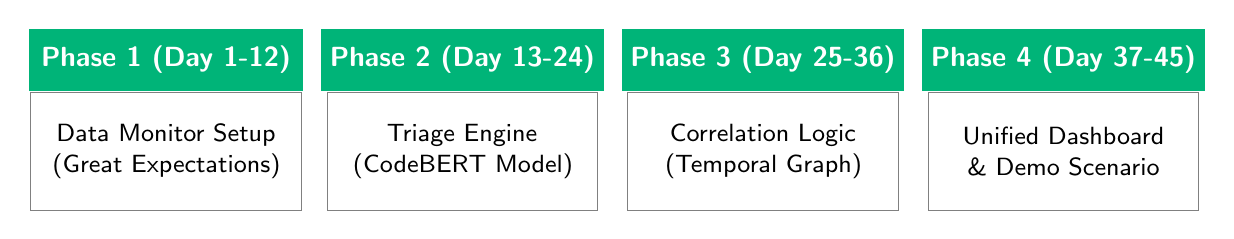
\begin{tikzpicture}[
        node distance=0cm,
        phase/.style={rectangle, draw=white, fill=UniGreen, text=white, font=\bfseries, minimum width=3.5cm, minimum height=0.8cm},
        task/.style={rectangle, draw=gray, fill=white, text width=3.2cm, align=center, font=\small, minimum height=1.5cm, anchor=north}
    ]
        \node[phase] (p1) {Phase 1 (Day 1-12)};
        \node[phase, right=0.2cm of p1] (p2) {Phase 2 (Day 13-24)};
        \node[phase, right=0.2cm of p2] (p3) {Phase 3 (Day 25-36)};
        \node[phase, right=0.2cm of p3] (p4) {Phase 4 (Day 37-45)};

        \node[task] at (p1.south) {Data Monitor Setup\\(Great Expectations)};
        \node[task] at (p2.south) {Triage Engine\\(CodeBERT Model)};
        \node[task] at (p3.south) {Correlation Logic\\(Temporal Graph)};
        \node[task] at (p4.south) {Unified Dashboard\\\& Demo Scenario};
    \end{tikzpicture}
\end{figure}

\section*{Conclusion}
\addcontentsline{toc}{section}{Conclusion}
DataBug AI transforms bug triage from a reactive, siloed process into a data-aware, intelligent system. By connecting the dots between data pipeline health and downstream bugs, we enable Unifonic to \textbf{stop treating symptoms and start finding root causes.}

\vspace{1cm}
\begin{center}
\begin{tcolorbox}[colback=UniGreen!10, colframe=UniGreen, width=10cm]
\centering
\Large\textbf{Stop treating symptoms.}\\
\Large\textbf{Start finding root causes.}
\end{tcolorbox}
\end{center}

%--- REFERENCES ---
\section*{References}
\addcontentsline{toc}{section}{References}

\begin{enumerate}[label={[\arabic*]}]
    \item DataChecks. (2024). \textit{The State of Data Quality 2024: Analysis of 1,000 Data Pipelines}. \url{https://www.datachecks.io/}

    \item Precisely. (2024). \textit{2025 Planning Insights: Data Quality Remains the Top Data Integrity Challenge}. \url{https://www.precisely.com/}

    \item Hevo Data. (2024). \textit{Common Data Pipeline Failures}. \url{https://hevodata.com/}

    \item Atlan. (2025). \textit{Open Source Data Quality Tools 2025}. \url{https://atlan.com/}

    \item Great Expectations. \textit{Documentation}. \url{https://docs.greatexpectations.io/}

    \item AWS Labs. \textit{Deequ: Data Quality Validation for Apache Spark}. GitHub. \url{https://github.com/awslabs/deequ}

    \item Mani, S., et al. (2019). \textit{DeepTriage: Exploring the Effectiveness of Deep Learning for Bug Triaging}. arXiv:1911.03657.

    \item DataKitchen. (2024). \textit{The Open-Source Data Quality and Data Observability Landscape}. \url{https://datakitchen.io/}
\end{enumerate}

\vfill
\begin{center}
\rule{0.5\textwidth}{0.4pt}\\
\vspace{0.3cm}
\textbf{Team CSIS} -- Unifonic AI Hackathon 2025
\end{center}

\end{document}
